% Generated by Sphinx.
\def\sphinxdocclass{report}
\documentclass[letterpaper,11pt,ngerman]{andi}
\usepackage[utf8]{inputenc}
\DeclareUnicodeCharacter{00A0}{\nobreakspace}
\usepackage{cmap}
\usepackage[T1]{fontenc}
\usepackage{babel}
\usepackage{times}
\usepackage[Sonny]{fncychap}
\usepackage{longtable}
\usepackage{sphinx}
\usepackage{multirow}
\usepackage{acronym}
%\usepackage[]{thumb}
%\usepackage{quotchap}
\usepackage{pdfpages}
\usepackage{remreset}
%\usepackage{bibunits}
\usepackage{extramarks}
%\usepackage{quotchap}
\usepackage{epigraph}
%\setcounter{tocdepth}{0}

\title{Literaturrecherche}
\date{13.08.2015}
\release{master}
\author{Dipl.-Ing. (FH) Andreas Gschossmann}
\newcommand{\sphinxlogo}{
\includegraphics{logo_oth.pdf}\par}
\renewcommand{\releasename}{Release}
\makeindex

\makeatletter
\def\PYG@reset{\let\PYG@it=\relax \let\PYG@bf=\relax%
    \let\PYG@ul=\relax \let\PYG@tc=\relax%
    \let\PYG@bc=\relax \let\PYG@ff=\relax}
\def\PYG@tok#1{\csname PYG@tok@#1\endcsname}
\def\PYG@toks#1+{\ifx\relax#1\empty\else%
    \PYG@tok{#1}\expandafter\PYG@toks\fi}
\def\PYG@do#1{\PYG@bc{\PYG@tc{\PYG@ul{%
    \PYG@it{\PYG@bf{\PYG@ff{#1}}}}}}}
\def\PYG#1#2{\PYG@reset\PYG@toks#1+\relax+\PYG@do{#2}}

\expandafter\def\csname PYG@tok@gd\endcsname{\def\PYG@tc##1{\textcolor[rgb]{0.63,0.00,0.00}{##1}}}
\expandafter\def\csname PYG@tok@gu\endcsname{\let\PYG@bf=\textbf\def\PYG@tc##1{\textcolor[rgb]{0.50,0.00,0.50}{##1}}}
\expandafter\def\csname PYG@tok@gt\endcsname{\def\PYG@tc##1{\textcolor[rgb]{0.00,0.27,0.87}{##1}}}
\expandafter\def\csname PYG@tok@gs\endcsname{\let\PYG@bf=\textbf}
\expandafter\def\csname PYG@tok@gr\endcsname{\def\PYG@tc##1{\textcolor[rgb]{1.00,0.00,0.00}{##1}}}
\expandafter\def\csname PYG@tok@cm\endcsname{\let\PYG@it=\textit\def\PYG@tc##1{\textcolor[rgb]{0.25,0.50,0.56}{##1}}}
\expandafter\def\csname PYG@tok@vg\endcsname{\def\PYG@tc##1{\textcolor[rgb]{0.73,0.38,0.84}{##1}}}
\expandafter\def\csname PYG@tok@m\endcsname{\def\PYG@tc##1{\textcolor[rgb]{0.13,0.50,0.31}{##1}}}
\expandafter\def\csname PYG@tok@mh\endcsname{\def\PYG@tc##1{\textcolor[rgb]{0.13,0.50,0.31}{##1}}}
\expandafter\def\csname PYG@tok@cs\endcsname{\def\PYG@tc##1{\textcolor[rgb]{0.25,0.50,0.56}{##1}}\def\PYG@bc##1{\setlength{\fboxsep}{0pt}\colorbox[rgb]{1.00,0.94,0.94}{\strut ##1}}}
\expandafter\def\csname PYG@tok@ge\endcsname{\let\PYG@it=\textit}
\expandafter\def\csname PYG@tok@vc\endcsname{\def\PYG@tc##1{\textcolor[rgb]{0.73,0.38,0.84}{##1}}}
\expandafter\def\csname PYG@tok@il\endcsname{\def\PYG@tc##1{\textcolor[rgb]{0.13,0.50,0.31}{##1}}}
\expandafter\def\csname PYG@tok@go\endcsname{\def\PYG@tc##1{\textcolor[rgb]{0.20,0.20,0.20}{##1}}}
\expandafter\def\csname PYG@tok@cp\endcsname{\def\PYG@tc##1{\textcolor[rgb]{0.00,0.44,0.13}{##1}}}
\expandafter\def\csname PYG@tok@gi\endcsname{\def\PYG@tc##1{\textcolor[rgb]{0.00,0.63,0.00}{##1}}}
\expandafter\def\csname PYG@tok@gh\endcsname{\let\PYG@bf=\textbf\def\PYG@tc##1{\textcolor[rgb]{0.00,0.00,0.50}{##1}}}
\expandafter\def\csname PYG@tok@ni\endcsname{\let\PYG@bf=\textbf\def\PYG@tc##1{\textcolor[rgb]{0.84,0.33,0.22}{##1}}}
\expandafter\def\csname PYG@tok@nl\endcsname{\let\PYG@bf=\textbf\def\PYG@tc##1{\textcolor[rgb]{0.00,0.13,0.44}{##1}}}
\expandafter\def\csname PYG@tok@nn\endcsname{\let\PYG@bf=\textbf\def\PYG@tc##1{\textcolor[rgb]{0.05,0.52,0.71}{##1}}}
\expandafter\def\csname PYG@tok@no\endcsname{\def\PYG@tc##1{\textcolor[rgb]{0.38,0.68,0.84}{##1}}}
\expandafter\def\csname PYG@tok@na\endcsname{\def\PYG@tc##1{\textcolor[rgb]{0.25,0.44,0.63}{##1}}}
\expandafter\def\csname PYG@tok@nb\endcsname{\def\PYG@tc##1{\textcolor[rgb]{0.00,0.44,0.13}{##1}}}
\expandafter\def\csname PYG@tok@nc\endcsname{\let\PYG@bf=\textbf\def\PYG@tc##1{\textcolor[rgb]{0.05,0.52,0.71}{##1}}}
\expandafter\def\csname PYG@tok@nd\endcsname{\let\PYG@bf=\textbf\def\PYG@tc##1{\textcolor[rgb]{0.33,0.33,0.33}{##1}}}
\expandafter\def\csname PYG@tok@ne\endcsname{\def\PYG@tc##1{\textcolor[rgb]{0.00,0.44,0.13}{##1}}}
\expandafter\def\csname PYG@tok@nf\endcsname{\def\PYG@tc##1{\textcolor[rgb]{0.02,0.16,0.49}{##1}}}
\expandafter\def\csname PYG@tok@si\endcsname{\let\PYG@it=\textit\def\PYG@tc##1{\textcolor[rgb]{0.44,0.63,0.82}{##1}}}
\expandafter\def\csname PYG@tok@s2\endcsname{\def\PYG@tc##1{\textcolor[rgb]{0.25,0.44,0.63}{##1}}}
\expandafter\def\csname PYG@tok@vi\endcsname{\def\PYG@tc##1{\textcolor[rgb]{0.73,0.38,0.84}{##1}}}
\expandafter\def\csname PYG@tok@nt\endcsname{\let\PYG@bf=\textbf\def\PYG@tc##1{\textcolor[rgb]{0.02,0.16,0.45}{##1}}}
\expandafter\def\csname PYG@tok@nv\endcsname{\def\PYG@tc##1{\textcolor[rgb]{0.73,0.38,0.84}{##1}}}
\expandafter\def\csname PYG@tok@s1\endcsname{\def\PYG@tc##1{\textcolor[rgb]{0.25,0.44,0.63}{##1}}}
\expandafter\def\csname PYG@tok@gp\endcsname{\let\PYG@bf=\textbf\def\PYG@tc##1{\textcolor[rgb]{0.78,0.36,0.04}{##1}}}
\expandafter\def\csname PYG@tok@sh\endcsname{\def\PYG@tc##1{\textcolor[rgb]{0.25,0.44,0.63}{##1}}}
\expandafter\def\csname PYG@tok@ow\endcsname{\let\PYG@bf=\textbf\def\PYG@tc##1{\textcolor[rgb]{0.00,0.44,0.13}{##1}}}
\expandafter\def\csname PYG@tok@sx\endcsname{\def\PYG@tc##1{\textcolor[rgb]{0.78,0.36,0.04}{##1}}}
\expandafter\def\csname PYG@tok@bp\endcsname{\def\PYG@tc##1{\textcolor[rgb]{0.00,0.44,0.13}{##1}}}
\expandafter\def\csname PYG@tok@c1\endcsname{\let\PYG@it=\textit\def\PYG@tc##1{\textcolor[rgb]{0.25,0.50,0.56}{##1}}}
\expandafter\def\csname PYG@tok@kc\endcsname{\let\PYG@bf=\textbf\def\PYG@tc##1{\textcolor[rgb]{0.00,0.44,0.13}{##1}}}
\expandafter\def\csname PYG@tok@c\endcsname{\let\PYG@it=\textit\def\PYG@tc##1{\textcolor[rgb]{0.25,0.50,0.56}{##1}}}
\expandafter\def\csname PYG@tok@mf\endcsname{\def\PYG@tc##1{\textcolor[rgb]{0.13,0.50,0.31}{##1}}}
\expandafter\def\csname PYG@tok@err\endcsname{\def\PYG@bc##1{\setlength{\fboxsep}{0pt}\fcolorbox[rgb]{1.00,0.00,0.00}{1,1,1}{\strut ##1}}}
\expandafter\def\csname PYG@tok@kd\endcsname{\let\PYG@bf=\textbf\def\PYG@tc##1{\textcolor[rgb]{0.00,0.44,0.13}{##1}}}
\expandafter\def\csname PYG@tok@ss\endcsname{\def\PYG@tc##1{\textcolor[rgb]{0.32,0.47,0.09}{##1}}}
\expandafter\def\csname PYG@tok@sr\endcsname{\def\PYG@tc##1{\textcolor[rgb]{0.14,0.33,0.53}{##1}}}
\expandafter\def\csname PYG@tok@mo\endcsname{\def\PYG@tc##1{\textcolor[rgb]{0.13,0.50,0.31}{##1}}}
\expandafter\def\csname PYG@tok@mi\endcsname{\def\PYG@tc##1{\textcolor[rgb]{0.13,0.50,0.31}{##1}}}
\expandafter\def\csname PYG@tok@kn\endcsname{\let\PYG@bf=\textbf\def\PYG@tc##1{\textcolor[rgb]{0.00,0.44,0.13}{##1}}}
\expandafter\def\csname PYG@tok@o\endcsname{\def\PYG@tc##1{\textcolor[rgb]{0.40,0.40,0.40}{##1}}}
\expandafter\def\csname PYG@tok@kr\endcsname{\let\PYG@bf=\textbf\def\PYG@tc##1{\textcolor[rgb]{0.00,0.44,0.13}{##1}}}
\expandafter\def\csname PYG@tok@s\endcsname{\def\PYG@tc##1{\textcolor[rgb]{0.25,0.44,0.63}{##1}}}
\expandafter\def\csname PYG@tok@kp\endcsname{\def\PYG@tc##1{\textcolor[rgb]{0.00,0.44,0.13}{##1}}}
\expandafter\def\csname PYG@tok@w\endcsname{\def\PYG@tc##1{\textcolor[rgb]{0.73,0.73,0.73}{##1}}}
\expandafter\def\csname PYG@tok@kt\endcsname{\def\PYG@tc##1{\textcolor[rgb]{0.56,0.13,0.00}{##1}}}
\expandafter\def\csname PYG@tok@sc\endcsname{\def\PYG@tc##1{\textcolor[rgb]{0.25,0.44,0.63}{##1}}}
\expandafter\def\csname PYG@tok@sb\endcsname{\def\PYG@tc##1{\textcolor[rgb]{0.25,0.44,0.63}{##1}}}
\expandafter\def\csname PYG@tok@k\endcsname{\let\PYG@bf=\textbf\def\PYG@tc##1{\textcolor[rgb]{0.00,0.44,0.13}{##1}}}
\expandafter\def\csname PYG@tok@se\endcsname{\let\PYG@bf=\textbf\def\PYG@tc##1{\textcolor[rgb]{0.25,0.44,0.63}{##1}}}
\expandafter\def\csname PYG@tok@sd\endcsname{\let\PYG@it=\textit\def\PYG@tc##1{\textcolor[rgb]{0.25,0.44,0.63}{##1}}}

\def\PYGZbs{\char`\\}
\def\PYGZus{\char`\_}
\def\PYGZob{\char`\{}
\def\PYGZcb{\char`\}}
\def\PYGZca{\char`\^}
\def\PYGZam{\char`\&}
\def\PYGZlt{\char`\<}
\def\PYGZgt{\char`\>}
\def\PYGZsh{\char`\#}
\def\PYGZpc{\char`\%}
\def\PYGZdl{\char`\$}
\def\PYGZhy{\char`\-}
\def\PYGZsq{\char`\'}
\def\PYGZdq{\char`\"}
\def\PYGZti{\char`\~}
% for compatibility with earlier versions
\def\PYGZat{@}
\def\PYGZlb{[}
\def\PYGZrb{]}
\makeatother

\begin{document}
\shorthandoff{"}
\maketitle
\tableofcontents
\phantomsection\label{index::doc}

\setcounter{tocdepth}{2}

\chapter{GPS}
\label{index:welcome-to-mergedocs-s-documentation}\label{index:gps}

\section{Grundlagen Globale Navigationssysteme (GNSS)}
\label{included_projects/gps/GPS_SPEC/content::doc}\label{included_projects/gps/GPS_SPEC/content:grundlagen-globale-navigationssysteme-gnss}

\subsection{Funktionsprinzip GNSS}
\label{included_projects/gps/GPS_SPEC/content:funktionsprinzip-gnss}
Jeder Satellit enthält eine hochgenaue Uhr. Er sendet das aktuelle Zeitsignal zur Erde. Die Uhr des Satelliten synchronisiert sich mit der Uhr des Empfänger- Moduls. Aus der Differenz der gesendeten Zeit und der Zeit beim Eintreffen des Signals kann die Laufzeit ermittelt werden. Über die Laufzeit und die Kenntnis, dass sich die Signale mit Lichtgeschwindigkeit ausbreiten kann schließlich der Abstand zur Erde ermittelt werden. \cite{sat_nav_schildt}
\begin{figure}[htbp]
\centering
\capstart

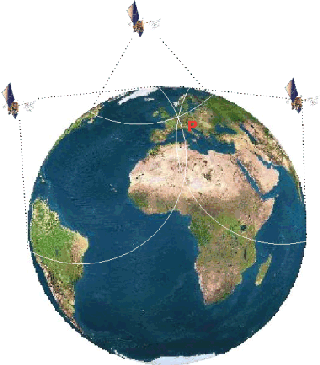
\includegraphics[width=0.350\linewidth]{gps_ranging.png}
\caption{Sateillitenortung \cite{fig_gps}}\end{figure}

Die mögliche Position, bezüglich eines Satelliten, liegt auf der Kugeloberfläche, aufgespannt durch die Lage des Satelliten, zum Sendezeitpunkt, als Mittelpunkt und dem ermittelten Abstand vom Satelliten als Radius. Aus dem Schnittpunkt von drei Kugeloberflächen ergeben zwei Schnittpunkte. Mit der Kenntnis der groben Lage, kann man einen der Schnittpunkte verwerfen. Es werden also mindestens drei Satelliten zur Ortung benötigt. Meist können auf der Erde jedoch ohnehin mehr Satelliten empfangen werden. \cite{sat_nav_schildt}


\subsection{Satellitensysteme}
\label{included_projects/gps/GPS_SPEC/content:satellitensysteme}

\subsubsection{NAVSTAR}
\label{included_projects/gps/GPS_SPEC/content:navstar}
Das NAVSTAR System wurde 1973 von den Amerikanern für militärische Zwecke entwickelt. Aufgrund des hohen wirtschaftlichen Nutzens wurde es später für das zivile Leben freigeschaltet. Es sendet auf zwei Frequenzen:
\begin{itemize}
\item {} 
Standard Positioning Service (SPS): Frequenz L1 mit 1575,42 MHz und einer Wiederholrate von 1,023 MHZ

\item {} 
Precision Positioning Service (PPS): Frequenz L2 mit 1227,6 MHz und einer Wiederholrate von 10,23 MHz

\end{itemize}

Die Frequenz L1 ist für die zivile und die Frequenz L2 für militärische Nutzung bestimmt. \cite{sat_nav_dodel} Das Zeitsignal der militärische Frequenz L2 ist mit dem sogenanntem Y-Code verschlüsselt und zivilen Nutzern nicht zugänglich. \cite{sat_nav_thaller} Zwar ist die Ortung allein durch die militärische Frequenz ungenauer, doch nur durch den Empfang beider Frequenzen L1 und L2 kann man durch das Mehrfrequenzverfahren Mehrwege- und Ionosphärenfehler herausrechnen und erhält damit eine höhere Genauigkeit. \cite{sat_nav_dodel}

Seit der GPSII Generation werden zusätzlich das L2C und das L5 (1176.45MHz) Signal angeboten. Durch den Empfang von mehreren Frequenzen zur Positionsbestimmung steht nun ein PPS-Dienst mit Mehrfrequenzverfahren für den zivilen Nutzen zur Verfügung. \cite{sat_nav_dodel}, \cite{gps_world}

\textbf{Einschränkungen der freien Nutzung von GPS:}

Nachdem die L1 Frequenz unter Präsident Reagan für die zivile Nutzung freigegeben wurde, befand man sich noch im Kalten Krieg. Deshalb wurde der Inhalt der zivilen Frequenz L1 durch die sogenannte Selective Availability (S/A) Funktion künstlich verschlechtert, um im zivilen Bereich eine niedrigere Genauigkeit von nur 100 Metern zu erzielen. Dies entsprach der Genauigkeit des Russischem Satellitennavigationssystem GLONASS. Damit hatten die Militärs der USA einen Vorteil gegenüber Russland, man spricht vom Window of Vulnerability. Präsident Bill Clinton gab im Jahr 2000 dem Druck aus der Wirtschaft und den mittlerweile sehr zahlreichen zivilen GPS Nutzern nach und ging auf eine Empfehlung des damaligen Vizepräsidenten Al Gore, die Selective Availability Funktion abzuschalten, ein. \cite{sat_nav_dodel}
Ein erneutes Einschalten der Selective Availability Funktion, welche ausschließlich global einsetzbar ist, ist nicht geplant. Die Satelliten der GPSIII Generation besitzen diese Funktion garnicht mehr. \cite{sat_nav_dodel} Stattdessen wird der Empfang der zivilen GPS Frequenzen in Kriesengebieten durch Jamming und Spoofing lokal gestört. \cite{sat_nav_schildt} Darauf wird näher in Kapitel 2.2 eingegangen.


\subsubsection{GALILEO}
\label{included_projects/gps/GPS_SPEC/content:galileo}
Seit die zivile Nutzung von GPS möglich ist, wurde die Navigation durch GPS zunächst im Schiffs- und Flugverkehr später auch im Straßenverkehr durch immer mehr Anwendungen vereinnahmt. Der Vorschlag der Federal Aviation Administration (FAA) in den 90iger Jahren, das Global Positioning System weltweit zum Sole Means of Navigation \footnote{
Ein Sole Means Of Navigation System ist in der Luftfahrt ein Navigationssystem, welches die Kriterien Genauigkeit und Integrität ausreichend erfüllt.
} zu machen, veranlasste die EU dazu ein eigenes Satellitennavigationssystem aufzubauen. Man wollte einer Abhängigkeit durch ein Monopol der USA, im Bereich der GNSS-Dienste, entgehen. \cite{sat_nav_dodel}

Das Galileoprogramm wurde als Private Public Partnership (PPP) umgesetzt. Die Entwicklungskosten und die Kosten für den Aufbau teilen sich die EU und die ESA. \cite{sat_nav_dodel} Es war damals geplant den kommerziellen Vertrieb von Galileo an einen Konzessionär auszuschreiben welcher die Betriebskosten tragen sollte. Neben den kostenlosen Diensten sollten gebührenpflichtige Zusatz-Dienste angeboten werden und es sollten Gebühren beim Kauf von GPS-Modulen anfallen, durch welche der Konzessionär Geld verdienen konnte. Ein entscheidendes Leistungsmerkmal sollte die höhere Genauigkeit von Galileo gegenüber GPS sein. Dieser Vorteil gegenüber GPS wurde jedoch geschwächt, nachdem die USA die Selective Availability Funktion des GPS Systems abgeschaltet hat. Der wichtigste Dienst von Galileo, der Ortungsdienst, ist kostenfrei und die kostenpflichtigen Dienste sind für mögliche Kunden nicht so attraktiv, wie man es sich erhofft hatte. Private Investoren sind abgesprungen und die Betriebskosten von Galileo müssen vom Steuerzahler getragen werden.

\textbf{Kritik an Galileo}

Da Galileo gegenüber GPS keinen marginal höheren Nutzen bringt erntet das
Projekt Kritik in den Medien: Die \emph{Süddeutsche Zeitung} schreibt kurz vor dem Start der ersten beiden Satelliten im Oktober 2012 in einem Kommentar: \emph{”Das Vorzeigeprojekt, das frühestens 2014 in einem rudimentären Zustand in Betrieb gehen wird, kommt Jahre zu spät, ist zu teuer und - verglichen mit den Konkurrenzsystemen - nicht gut genug.“} \cite{galileo_fail} Etwa zeitgleich schreibt die Die Zeit Online: \emph{”Der Raumfahrt-Forscher und ehe- malige Astronaut Ulrich Walter von der Technischen Universität München hält dagegen, dass Galileo für gewöhnliche Anwender wie Autofahrer keine Verbesserung bringe.“} \cite{galileo_start} Der hohe finanzielle Aufwand, welcher nur geringen finanziellen Einnahmen gegenüber steht und vom Steuerzahler getragen werden muss, steht unter Kritik. Laut Spiegel Online, im Januar 2011, \emph{”veranschlagt die europäische Komission für den Aufbau der Infrastruktur bis 2020 rund 5,3 Milliarden Euro, das sind 1,9 Milliarden Euro zusätzlich.“} \cite{gal_exp} Auch die laufenden Kosten in Höhe von jährlich 800 Millionen Euro müssen vom Steuerzahler getragen werden.

Ein Kritikpunkt an dem technischen Konzept von Galileo ist, dass es lediglich ein Nachbau der veralteten GPS Technik sei. Alle Satelliten senden auf den selben Frequenzen, mit den selben technischen Nachteilen. Das Signal darf nicht zu Leistungsstark sein, damit die anderen Satelliten nicht übertönt werden können. Dadurch ist das Signal auf der L1 und L2 Frequenz relativ schwach. Dieser Nachteil kann jedoch ebenfalls als Vorteil gesehen werden, da Galileo damit komplett kompatibel zu GPS ist. Deshalb werden keine eigenen Receiver benötigt und die weltweite Verfügbarkeit von GNSS wird insgesamt erhöht.

\textbf{Vorteile von Galileo:}
Trotz der Kritik bietet Galileo einige Vorteile. Für Galileo spricht, dass Europa in der Navigation unabhängig vom amerikanischen und Russischen Militär ist. Man hat in der Vergangenheit gesehen wie einfach die USA, durch Aktivierung der Selective Availability Funktion, die Genauigkeit von GPS global verschlechtern konnte und man wollte solchen politischen Entscheidungen nicht hilflos ausgeliefert sein. Ein anderer Vorteil von Galileo ist die Möglichkeit die empfangenen Signale auf Integrität zu prüfen. Damit ist der Weg geebnet Galileo für sicherheitsrelevante Anwendungen, wie beispielsweise der Navigation im Flugverkehr, anzuwenden. Außerdem ist Galileo kompatibel zu GPS. Damit wird die Verfügbarkeit der Ortungsdienste erhöht. Zusätzlich wird durch Mehrfrequenzverfahren (... L1 L2 L5) die Genauigkeit der Ortung erhöht und damit ist ein PPS Dienst für den zivilen Nutzen verfügbar.

\textbf{Dienste von Galileo:}

”Im Galileo-System werden voraussichtlich fünf Dienste auf fünf Frequenzen angeboten:
\begin{itemize}
\item {} 
Der gebührenfreie Basisdienst (Open Service, OS) ohne Chiffrierung: Positions- und Zeitsignale des Systems erlauben bei Verwendung eines Zweifrequenzempfängers eine Positionsbestimmung von 4 m Genauigkeit (lateral).

\item {} 
Der kommerzielle Dienst (Commercial Service, CS) mit Chiffrierung: bietet gegen Gebühr Genauigkeiten bis um einen Meter; Empfangssicherheit ist wie bei allen Diensten in Häuserschluchten und innerhalb von Gebäuden physikalisch begrenzt.

\item {} 
Der sicherheitskritische Dienst (Safety-of-Life-Service, SoL), garantierter Dienst: beinhaltet die Galileo-Funktionsüberwachung in Form eines systeminternen Integritätsdienstes und wird im Luft-, See- und Schienenverkehr eingesetzt.

\item {} 
Der öffentlich regulierte Dienst (Public Regulated Service, PRS), mit häufig wechselndem Schlüssel chiffriert: wird Militär, Polizei, und Rettungsdiensten vorbehalten.

\item {} 
Der Such- und Rettungsdienst (Search and Rescue Service, SAR6): die Übermittlung von Notsignalen, die die Koordinaten des Havaristen beinhalten, an Rettungsdienste nahezu in Echtzeit.“ \cite{sat_nav_dodel}

\end{itemize}
%\vfill
\vspace{0.5cm}

\begin{threeparttable}
\capstart\caption{Dienste, angeboten von Galileo und die Zuordnung zu den jeweiligen Frequenzen [3]} \label{tablelang}

\begin{tabular}{rllllllll}
   \hline
   %& \textit{L1/E1} & \textit{E5a} & \textit{E5b} & \textit{E6} & \textit{L-Band} & \textit{P-Band} \\ \hline
   &Art des Dienstes & \textit{L1/E1} & \textit{E5a} & \textit{E5b} & \textit{E6} & \textit{L-Band} & \textit{P-Band} \\
   &&1575,2&1176,45&1207,14&1278,75&1544,10&406,00&f [MHz] \\ \hline
   \textit{1}&\textit{Open Service}&\(\times\)&\(\times\)&\(\times\)&\(-\)&\(-\)&\(-\) \\
   \textit{2}&\textit{Commercial Service}&\(\times\)&\(-\)&\(\times\)&\(\times\)& \(-\) & \(-\) \\
   \textit{3}&\textit{Safety of Life}&\(\times\)&\(\times\)&\(\times\)&\(-\)& \(-\) & \(-\) \\
   \textit{4}&\textit{Public Regulated}&\(\times\)&\(-\)&\(-\)&\(\times\)& \(-\) & \(-\) \\
   \textit{5}&\textit{Search and Rescue}&\(-\)&\(-\)&\(-\)&\(-\)& \(\times\)  & \(\times\) \\
   &\textit{Intefity Information}&\(-\)&\(-\)&\(\times\)&\(-\)& \(-\) & \(-\) \\
   \hline
\end{tabular}
%\tiny
%\(\bullet\) Native Unterstützung in vollem Umfang\newline
%\(\circ\) Nur bedingte Unterstützung durch verschiedene Autoren mit ungewisser Maintainance, möglicherweise mit eingeschränktem Funktionsumfang

\end{threeparttable}

%\vfill
\vspace{0.5cm}
\textbf{Einsatzbereitschaft von Galileo}

Die ersten Galileo-Sateliten wurden 2011 ins All geschossen. Bis Mai 2015 wurden 8 Satelliten ins All geschossen. 2016 sollen die ersten Galileo-Dienste zur Verfügung stehen, das gesamte Netz von 30 Satelliten soll bis 2020 fertiggestellt werden. Die Signale von Galileo sind kompatibel zu GPS. Es werden jedoch im Vergleich zu GPS noch weitere Dienste, wie etwa Echtzeit-Ortung von Notrufen angeboten. \cite{europe_galileo}


\subsubsection{Korrektursatellitensysteme EGNOS, WAAS und MSAS}
\label{included_projects/gps/GPS_SPEC/content:korrektursatellitensysteme-egnos-waas-und-msas}
Für das GPS System gibt es jeweils für den amerikanischen, europäischen und asiatischen Raum Korrektursatellitensysteme:
\begin{itemize}
\item {} 
WAAS, Wide Area Augmentation System: Amerika

\item {} 
EGNOS, European Geostationary Navigation Overlay System: Europa

\item {} 
MSAS, Multi-Functional Satellite Augmentation System: Asien, vorwiegend Japan

\end{itemize}

Diese Satellitengestützten Systeme senden Korrektursignale, welche die Positionsgenauigkeit von GPS-Empfängern verbessern. Zusammen nennt man sie Satellite Based Augmentation Systems (SBAS) \cite{env_stud} Die Korrektursignale werden über Differential GPS (D-GPS) berechnet. \cite{sat_nav_schildt}

Die Funktionsweise von Differential GPS besteht darin, einen ortsfesten GPS-Empfänger in einer Referenzstation zu installieren, dessen Position man genau kennt. Dieser ortsfeste GPS-Empfänger misst die Laufzeit zu allen sichtbaren GPS-Satelliten. Mit der Kenntnis der wahren Position berechnet diese Referenzstation die Differenz zwischen Istwert und Sollwert der Laufzeiten. Die Differenzwerte werden via der Korrektursatelliten an den GPS Nutzer gesendet. Befindet sich der GPS Nutzer in der Nähe der Referenzstation ist davon auszugehen, dass die Abweichung der Laufzeiten, der jeweiligen Satelliten ähnlich sind. Damit kann der Nutzer mit den Differenzwerten die eigene Postion korrigieren und erhält ein genaueres Positionssignal. \cite{sat_nav_schildt}

Die Satellitenkorrektursysteme befinden sich in der ersten Testphase, können aber bereits empfangen werden. Sie werden weiterhin ausgebaut. Auch für Galileo und GLONASS existieren ähnliche Systeme, diese sind jedoch noch nicht so ausgereift, wie die genannten GPS-Korrektursysteme. \cite{sat_nav_schildt}

\textbf{Probleme beim Empfang von SBAS Signalen in Deutschland:}

Jener SBAS-Satellit, welcher in Deutschland am besten empfangen werden kann befindet sich sehr weit südlich, nahe am Horizont. Deshalb kann es sehr leicht zu Abschattungen kommen. \cite{sat_nav_schildt}

Jedoch ist es nicht zwingend notwendig, Korrekturdaten von den genannten SBAS-Systemen zu beziehen. Alternativ können diese vom \emph{Bundesamt für Kartographie und Geodäsie (BKG)} \footnote{
Das \emph{Bundesamt für Kartographie und Geodäsie (BKG)} betreibt zahlreiche Referenzstationen in ganz Deutschland.
} - über das Internet - bezogen werden. Eine weitere Möglichkeit besteht darin ortsfeste Referenzstationen mit GPS-Empfänger, deren exakte Position durch eine Mittelung der Positionsdaten über die Zeit gemessen werden, aufzustellen. Diese können dann aus deren bekannter Position Korrekturdaten ermitteln. Der Vorteil dieser Lösung ist, dass keine Verbindung zum Internet benötigt wird.


\subsection{Erhöhung der Präzision bei der Ortung}
\label{included_projects/gps/GPS_SPEC/content:erhohung-der-prazision-bei-der-ortung}
Der Trend der GNSS geht ohnehin in Richtung genauerer Messungen. Galileo und GPS haben ihre Dienste um eine weitere Frequenz, die L5-Frequenz, ausgebaut und bieten mittlerweile kostenlos Mehrfrequenzverfahren zur Kompensation des Ionosphärenfehlers an. Damit wird eine Genauigkeit von einigen Metern erreicht. \cite{podcast}

Eine Methode, die Genauigkeit zu Erhöhen ist die Verwendung von Differential GPS. Dabei wird ein GPS-Empfänger in einer Referenz-Station, mit bekanntem Ort untergebracht. Diese Referenzstation berechnet dann Korrektursignale. Diese werden an den jeweiligen GPS-Empfänger übertragen. Mittlerweile existieren auch Satellitensysteme, welche Korrektursignale von Bodenstationen übertragen. Da der Ionosphärenfehler über große räumliche Bereiche sehr ähnlich ist, gelten die ermittelten Referenzsignale für GPS-Empfänger, welche sich in der Nähe der Referenzstationen befinden. Dadurch können Genauigkeiten von unter einem Meter erreicht werden. \cite{podcast}

Ein Trick, die Genauigkeit zu erhöhen ist es, nicht das Zeitsignal zu ermitteln, sondern eine Phasenlaufzeitmessenung am Trägersignal durchzuführen. Dadurch kann man eine Genauigkeit erreichen, welche im Wellenlängenbereich des Trägersignals liegt. Dieses Verfahren ist jedoch teuer, da man sehr gute Antennen benötigt. \cite{podcast}

Auch durch die kombinierte Nutzung von Glonass und GPS/Galileo kann eine Verbesserung der Genauigkeit erreicht werden. Man kann mit beiden Systemen die Position erfassen und danach den Mittelwert bilden. Oft kommt es vor, dass sich die Abweichungen teilweise kompensieren.


\subsection{Sonstige Satellitengestützte Navigationssysteme}
\label{included_projects/gps/GPS_SPEC/content:sonstige-satellitengestutzte-navigationssysteme}
Das Russische Satellitensystem unterscheidet sich durch durch das Übertragungsprotokoll. Es wird für die Übertragung der Signale nicht die Code division multiple access (CDMA) Methode verwendet, sondern das sogenannte Frequency Division Multiple Access (FDMA) Verfahren. Dabei sendet jeder Satellit auf einer eigenen Frequenz und wird durch seine charakteristische Frequenz unterschieden.  Da das Russische System im Gegensatz zu Galileo nicht kompatibel zu GPS ist, ist es hierzulande etwas unbeliebter, da man eine zusätzliche Empfängertechnik benötigt, was teurer ist, als ein reiner GPS Empfänger. \cite{podcast}

Das Chinesische GNSS System heißt Kompass und befindet sich derzeit im Aufbau. Auch die Japaner und die Inder bauen lokale Ortungssysteme auf, welche GPS unterstützen.


\section{Einschränkung der Nutzung von GNSS-Diensten}
\label{included_projects/gps/GPS_SPEC/content:einschrankung-der-nutzung-von-gnss-diensten}

\subsection{Selective Availability (S/A)}
\label{included_projects/gps/GPS_SPEC/content:selective-availability-s-a}
Aus Gründen der nationalen Sicherheit wurde in den Anfängen der zivilen Nutzung das Frequenzband L1, welches für die zivile Nutzung zur Verfügung stand, künstlich verschlechtert. Die NAVSTAR/GPS Satelliten sendeten nicht das Signal ihrer Atomuhren. Stattdessen wurde ein Zeitsignal errechnet, welches innerhalb von bestimmten Grenzen vom korrekten Signal abweicht. Dieses abweichende Zeitsignal wurde anstelle des korrekten Zeitsignals gesendet. Diese Funktion nennt man Selective Availability (S/A). Sie ist nur global einsetzbar. \cite{sat_nav_dodel}

Aufgrund der wirtschaftlichen Vorteile von GPS ordnete Bill Clinton im Jahr 2000 die Abschaltung der S/A an. Seitdem ist GPS mit der Genauigkeit von unter zehn Metern für den zivilen Nutzen verfügbar. Eine erneute Aktivierung von S/A ist laut einer Erklärung von George W. Bush nicht vorgesehen. {[}5{]}

Da es mittlerweile Möglichkeiten gibt GPS lokal zu stören ist nicht davon auszugehen, dass S/A wieder eingeschaltet wird. Die letzte Generation von GPS (GPSIII) Satelliten bietet diese Funktion nicht mehr an. \cite{sat_nav_dodel}


\subsection{Lokale Täuschung durch Spoofing, Jamming, Meaconning}
\label{included_projects/gps/GPS_SPEC/content:lokale-tauschung-durch-spoofing-jamming-meaconning}
Mit den Methoden Spoofing, Jamming und Meaconing ist es möglich die Ortung durch GPS lokal zu stören. Das Signal von GPS zu emulieren und falsche Werte zu senden nennt man Spoofing. Bei Meaconing wird das GPS Signal aufgezeichnet und zeitversetzt gesendet. Das Übertönen des GPS Signals durch ein Signal gleicher Frequenz mit hinreichender Leistung nennt man Jamming.


\subsection{Geplante Einschränkungen}
\label{included_projects/gps/GPS_SPEC/content:geplante-einschrankungen}
Es ist geplant GNSS-Dienste ähnlich wie Pay-TV zu verschlüsseln. Zum einen können damit kostenpflichtige Dienste bei Bedarf selektiv freigeschaltet werden, zum anderen kann damit die Nutzung von GNSS-Diensten für Unbefugte vermieden werden. Es ist auch denkbar, dass die Schlüssel nicht individuell an die Nutzer verteilt werden, sondern landesspezifisch. Damit wäre eine Möglichkeit geschaffen, GNSS-Dienste lokal abzuschalten indem die GPS-Empfänger für bestimmte Länder diskriminiert werden. \cite{sat_nav_dodel}


\chapter{Rechtliches}
\label{index:rechtliches}

\section{Motivation}
\label{included_projects/rechtliches/RECHTLICHES_SPEC/content:motivation}\label{included_projects/rechtliches/RECHTLICHES_SPEC/content::doc}
Der Aufstieg eines Flugmodelles, oder eines unbemannten Fluggerätes bedeutet, dass man Teilnehmer des Flugverkehrs ist. Deshalb ist es nötig, geltendes deutsches Recht der Luftfahrt zu beachten.

\begin{notice}{note}{Bemerkung:}
Die Interpretation aller genannter Gesetze ist hier nicht durch einen Anwalt geschehen und sollte deshalb kritisch gesehen werden.
\end{notice}


\section{Geltendes Recht in der Luftfahrt}
\label{included_projects/rechtliches/RECHTLICHES_SPEC/content:geltendes-recht-in-der-luftfahrt}
Geltendes Recht, welches für Flugmodelle und unbemannte Fluggeräte gilt kann in folgenden Dokumenten nachgelesen werden:
\begin{itemize}
\item {} 
\href{http://www.gesetze-im-internet.de/luftvg/index.html}{LuftVG}, Luftverkehrsgesetz

\item {} 
\href{http://www.gesetze-im-internet.de/luftvo/}{LuftVO}, Luftvekehrsordnung

\item {} 
\href{http://www.gesetze-im-internet.de/luftvzo/}{LuftVZO}, Luftverkehrs-Zulassungs-Ordnung

\end{itemize}

Alle Gesetze wurden zuletzt am 8. Mai 2012 geändert.


\section{Nutzung des Luftraumes}
\label{included_projects/rechtliches/RECHTLICHES_SPEC/content:luftvzo}\label{included_projects/rechtliches/RECHTLICHES_SPEC/content:nutzung-des-luftraumes}
Am 8. Mai 2012 wurde das Luftverkehrsgesetz (\href{http://www.gesetze-im-internet.de/luftvg/index.html}{LuftVG}) geändert. Seit dem gelten ``unbemannte Fluggeräte einschließlich ihrer Kontrollstation, die nicht zu Zwecken des Sports oder der Freizeit betrieben werden (unbemannte Luftfahrtsysteme)'' (\href{http://www.gesetze-im-internet.de/luftvg/\_\_2.html}{\S{} 1 Abs. 2 LuftVG}) als Luftfahrzeuge und sind damit für die Benutzung des Luftraumes (\href{http://www.gesetze-im-internet.de/luftvg/\_\_1.html}{\S{} 1 Abs. 1 LuftVG}) freigegeben.

Fluggeräte, welche in geschlossenen Räumen oder Hallen betrieben werden, unterliegen nicht dem LuftVG, da sie nicht im öffentlichen deutschen Luftraum betrieben werden.


\section{Autonomer Flug}
\label{included_projects/rechtliches/RECHTLICHES_SPEC/content:autonomer-flug}\label{included_projects/rechtliches/RECHTLICHES_SPEC/content:autonomous}
``Der Luftfahrzeugführer hat zur Vermeidung von Zusammenstößen {[}...{]} einen ausreichenden Abstand einzuhalten.'' (\href{http://www.gesetze-im-internet.de/luftvo/\_\_12.html}{\S{}12 Abs. 1 LuftVO}) Entsprechende Regelungen für das Ausweichen werden in \href{http://www.gesetze-im-internet.de/luftvo/\_\_13.html}{\S{}13} der LuftVO definiert. Da diese Fähigkeit des Ausweichens einer autonomen Steuerung bisher nicht nachgewiesen wurde, kann man dies als implizites Verbot des autonomen Fluges deuten.

Außerdem ist ``der Betrieb von unbemannten Luftfahrtsystemen verboten, wenn {[}...{]} er außerhalb der Sichtweise des Steuerers erfolgt.'' (\S{}15a Abs. 3 LuftVO) Dabei muss die Sicht auf das Luftfahrtsystem ``ohne optische Hilfsmittel'' (\href{http://www.gesetze-im-internet.de/luftvo/\_\_15a.html}{\S{}15a Abs. 3 LuftVO}) möglich sein. Die Luftfahrtbehörde kann dieses Verbot jedoch aufheben. \(\rightarrow\) Genehmigungspflicht

Eine Regelung für den autonomen Flug im zivilen Bereich besteht derzeit noch nicht, es wird jedoch daran gearbeitet.


\section{Versicherungspflicht}
\label{included_projects/rechtliches/RECHTLICHES_SPEC/content:versicherungspflicht}\label{included_projects/rechtliches/RECHTLICHES_SPEC/content:a-abs-3-luftvo}
Nach \S{}102 der LuftVZO muss der Schaden der durch den Betreib eines Luftfahrzeuges entsteht versichert sein. Bei gewerblicher Nutzung ist zursätzlich darauf zu achten, dass eine gewerbliche Haftpflichtversicherung abgelegt wird.


\section{Gewicht eines unbemannten Luftfahrzeuges}
\label{included_projects/rechtliches/RECHTLICHES_SPEC/content:gewicht-eines-unbemannten-luftfahrzeuges}
Wiegt ein unbemanntes Luftfahrzeug mehr als 25 Kilogramm, ist dessen Betrieb nach \S{}15a Abs. 3 der LuftVO verboten.

\begin{notice}{note}{Bemerkung:}
Die allgemeine Aufstiegserlaubnis der jeweiligen Länder kann unter Umständen diese Grenze noch einmal auf 5 kg limitieren.
\end{notice}


\section{Fluggenehmigung}
\label{included_projects/rechtliches/RECHTLICHES_SPEC/content:fluggenehmigung}
``Luftfahrzeuge dürfen außerhalb der sie genehmigten Flugplätze nur starten und landen, wenn der Grundstückseigentümer oder sonst Berechtigte zugestimmt und die Luftfahrtbehörde eine Erlaubnis erteilt hat.'' (\S{} 25 Abs. 1 LuftVG)

\begin{notice}{note}{Bemerkung:}
Luftkarten beachten
\end{notice}

Außerdem gilt nach \S{}16 Abs. 1 der LuftVO, dass ``der Aufstieg von unbemannten Luftfahrtsystemen'' einer Erlaubnis bedarf.


\section{Luftaufnahmen}
\label{included_projects/rechtliches/RECHTLICHES_SPEC/content:luftaufnahmen}

\subsection{Verletzung des höchstpersönlichen Lebensbereichs}
\label{included_projects/rechtliches/RECHTLICHES_SPEC/content:verletzung-des-hochstpersonlichen-lebensbereichs}
Die ``Verletzung des höchstpersönlichen Lebensbereichs durch Bildaufnahmen'' wird mit bis zu einem Jahr Freiheitsstrafe geahndet. \cite{lebensbereich} \cite{heimlich} Dies trifft laut \S{}201 Abs. 1 StGB, dann ein, wenn heimlich Aufnahmen von Personen in ``gegen Einblick geschützten Räumen'' gemacht werden. Wörtlich heißt es hier:

``Wer von einer anderen Person, die sich in einer Wohnung oder einem gegen Einblick besonders geschützten Raum befindet, unbefugt Bildaufnahmen herstellt oder überträgt und dadurch deren höchstpersönlichen Lebensbereich verletzt, wird mit Freiheitsstrafe bis zu einem Jahr oder mit Geldstrafe bestraft.''

Würde man beispielsweise Aufnahmen von Leuten, die sich in einem durch eine undurchsichtige Hecke abgetrennten Garten sonnen, wäre der genannte Tatbestand erfüllt.


\subsection{Polizei}
\label{included_projects/rechtliches/RECHTLICHES_SPEC/content:polizei}
Die Aufnahmen von Demonstranten sind nur erlaubt, wenn Straftaten zu befürchten sind. Dies wurde per Gerichtsurteil entschieden. \cite{filmverbot}


\subsection{Recht am eigenen Bild}
\label{included_projects/rechtliches/RECHTLICHES_SPEC/content:recht-am-eigenen-bild}
Sind auf Bildern einzelne Personen eindeutig zu erkennen, ist die Veröffentlichung nur mit Einwilligung jener Personen erlaubt. Werden die Bilder ohne die Zustimmung der betroffenen Personen veröffentlicht, wird das verfassungrechtlich zugesicherte Persönlichkeitsrecht verletzt. Dies kann mit Geld- oder Freiheitsstrafen geahndet werden.


\subsection{Öffentlicher Raum}
\label{included_projects/rechtliches/RECHTLICHES_SPEC/content:offentlicher-raum}
Luftbilder vom öffentlichen Raum sind erlaubt.


\section{Flughöhe}
\label{included_projects/rechtliches/RECHTLICHES_SPEC/content:flughohe}
Siehe {\hyperref[included_projects/rechtliches/RECHTLICHES_SPEC/content:autonomous]{\emph{Autonomer Flug}}}.:
Die Drohne muss sich in Sichtweite des Piloten befinden.
\begin{appendix}
%\renewcommand{\chaptermark}[1]{\markboth{ \appendixname\ \thechapter ~ \ #1}{}}
\addcontentsline{toc}{chapter}{Anhang}\renewcommand\thechapter{\Alph{chapter}}

\chapter{GPS Artikel}
\label{index:gps-artikel}

\section{Zeitungsartikel}
\label{included_projects/gps/GPS_SPEC/appendix::doc}\label{included_projects/gps/GPS_SPEC/appendix:zeitungsartikel}
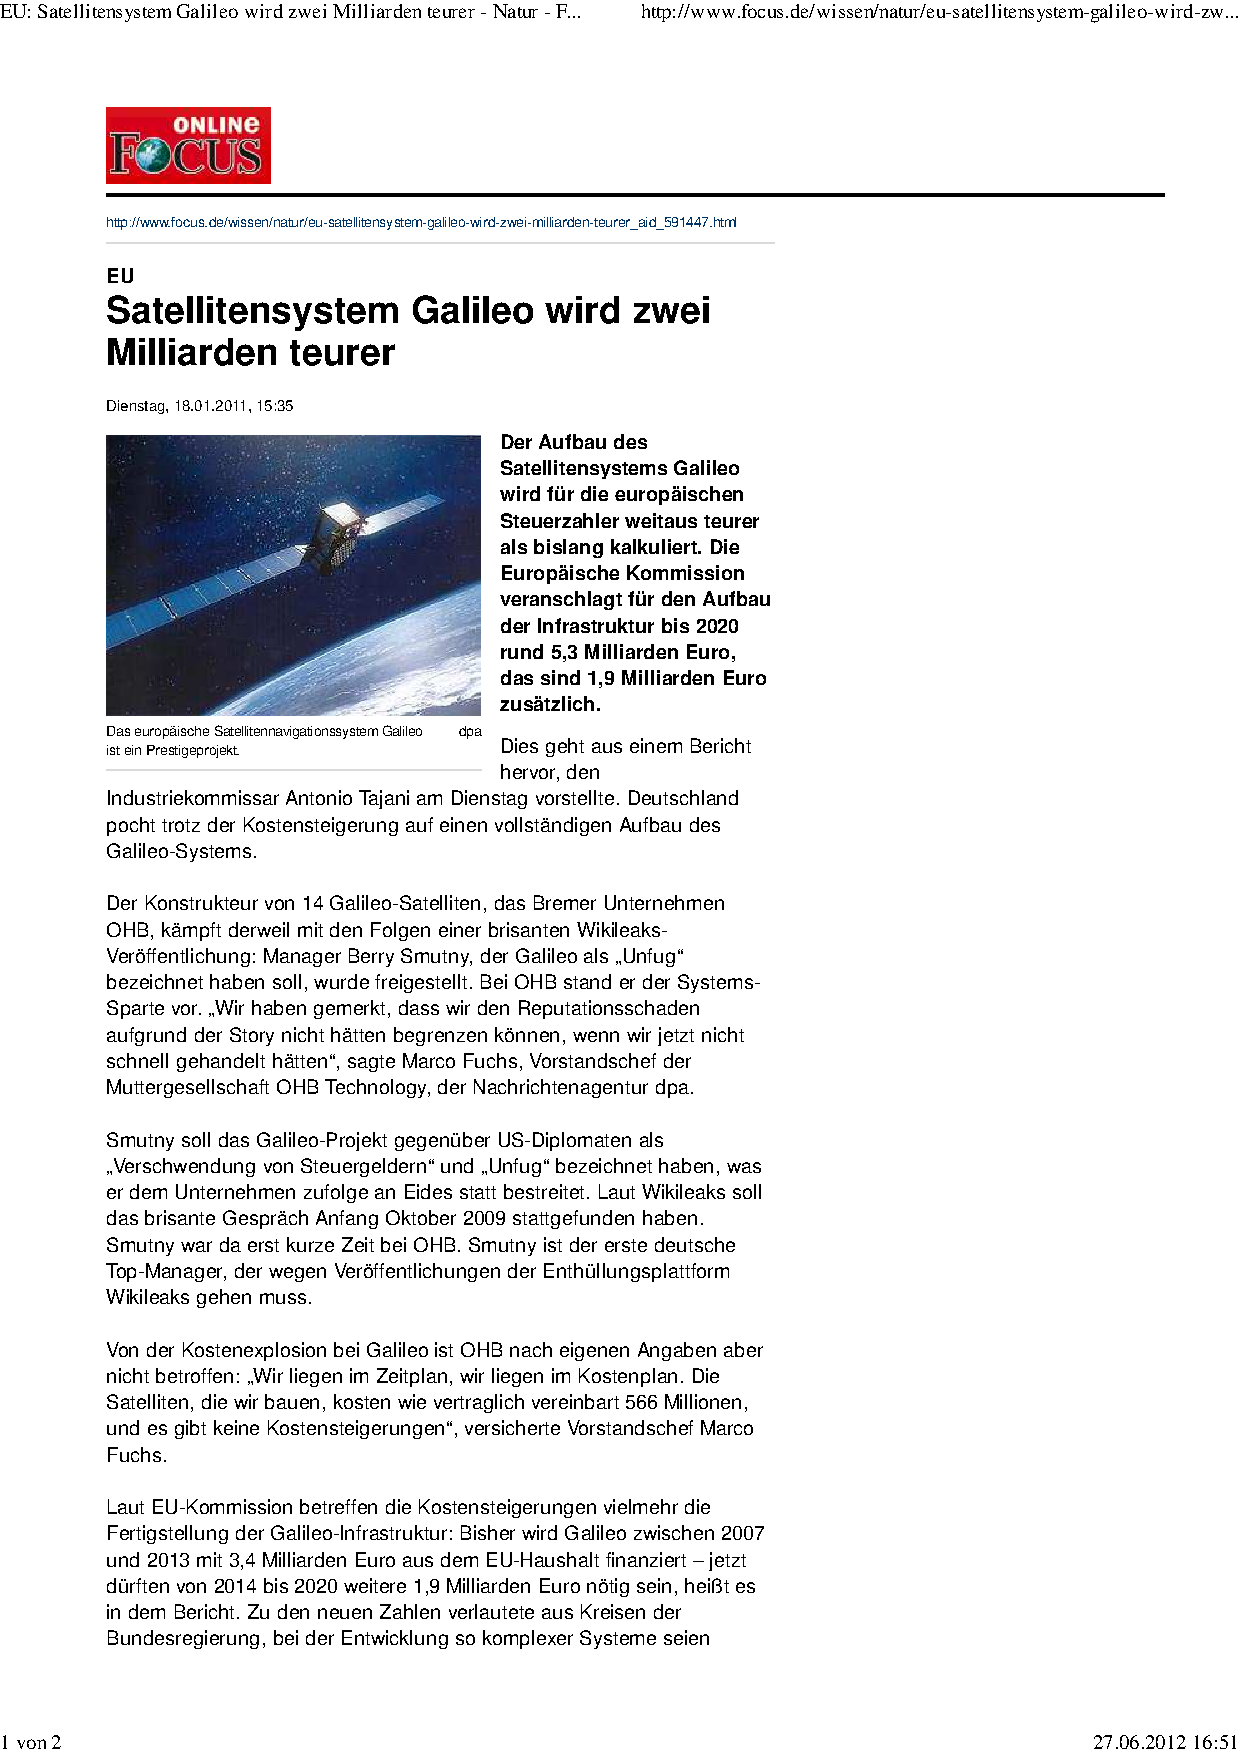
\includepdf[landscape=false, pages=-]{EU_Satellitensystem_Galileo_wird_zwei_Milliarden_teurer-Natur-FOCUS_Online-Nachrichten.pdf}

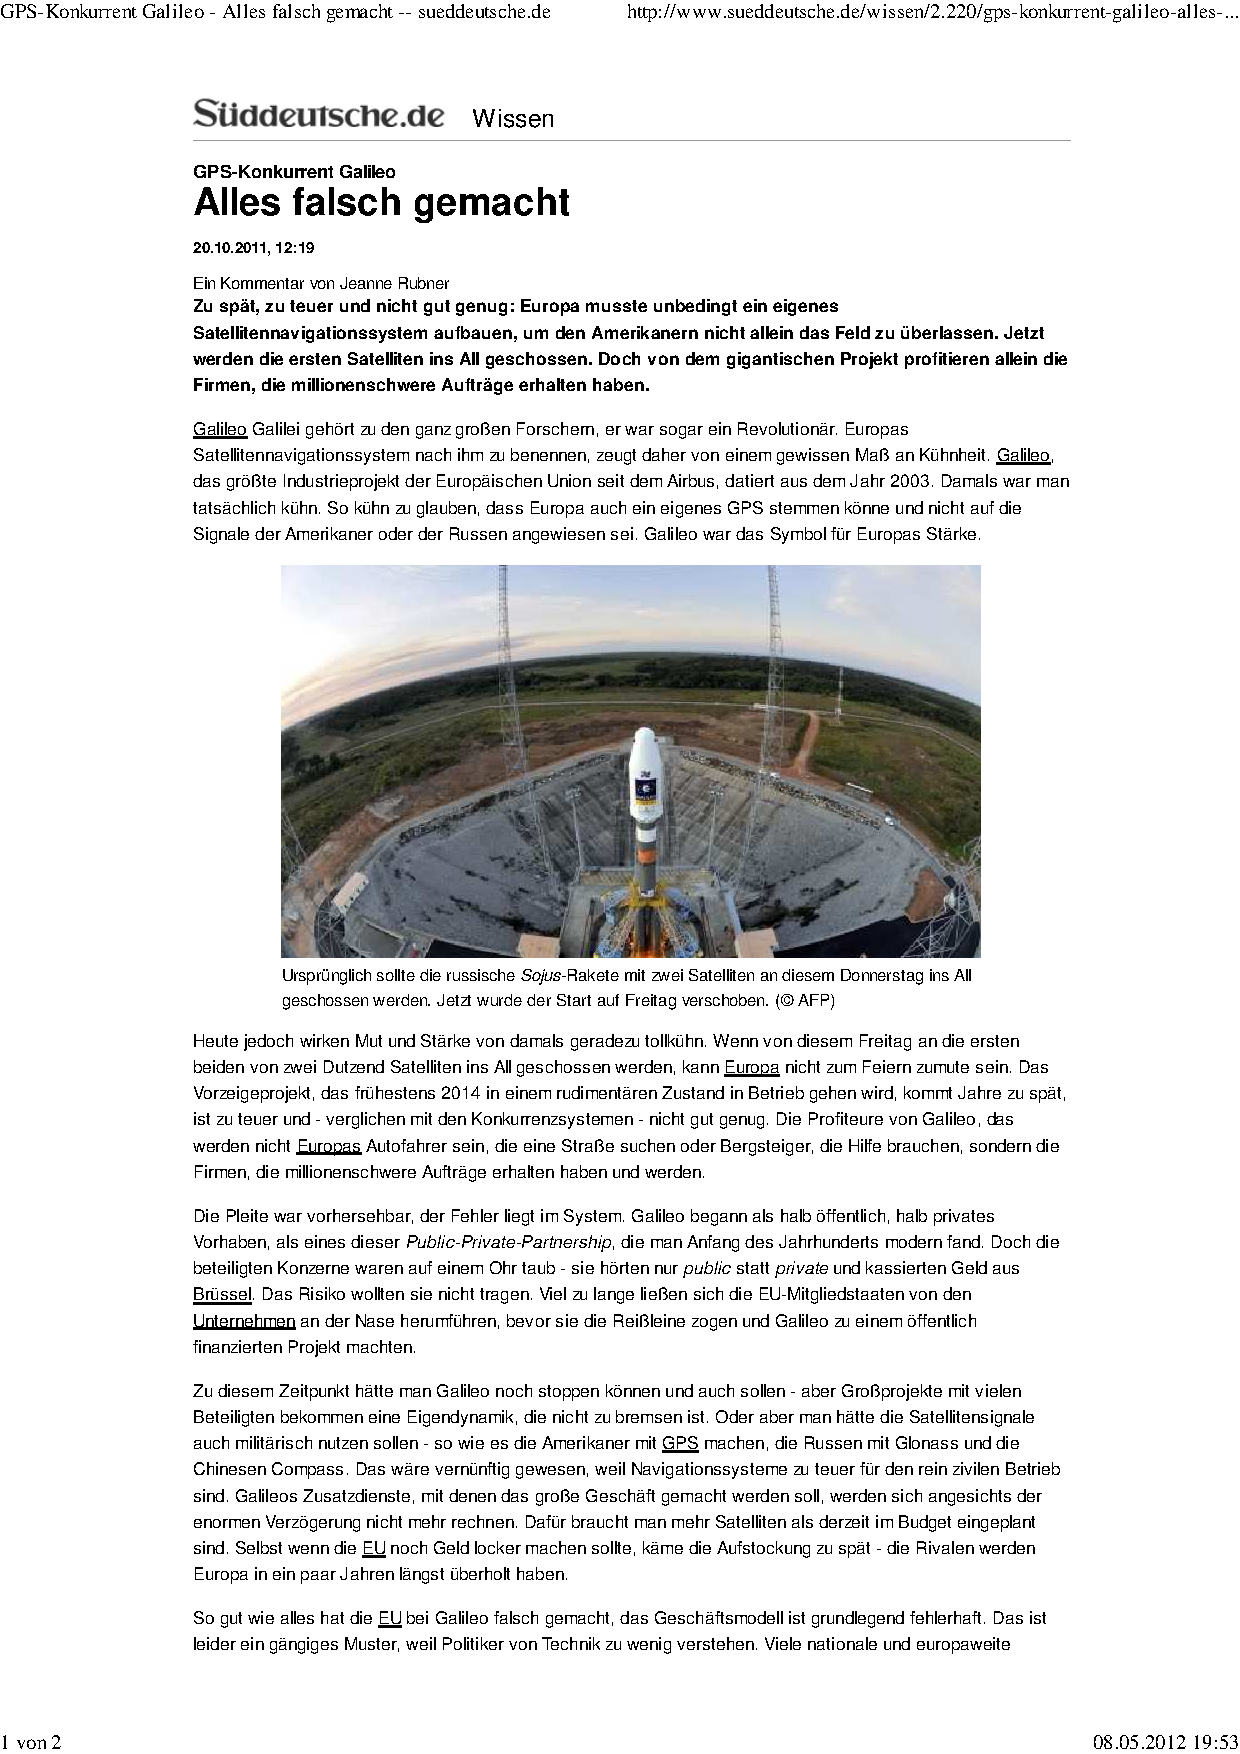
\includepdf[landscape=false, pages=-]{GPS-Konkurrent_Galileo-Alles_falsch_gemacht-sueddeutsche.pdf}

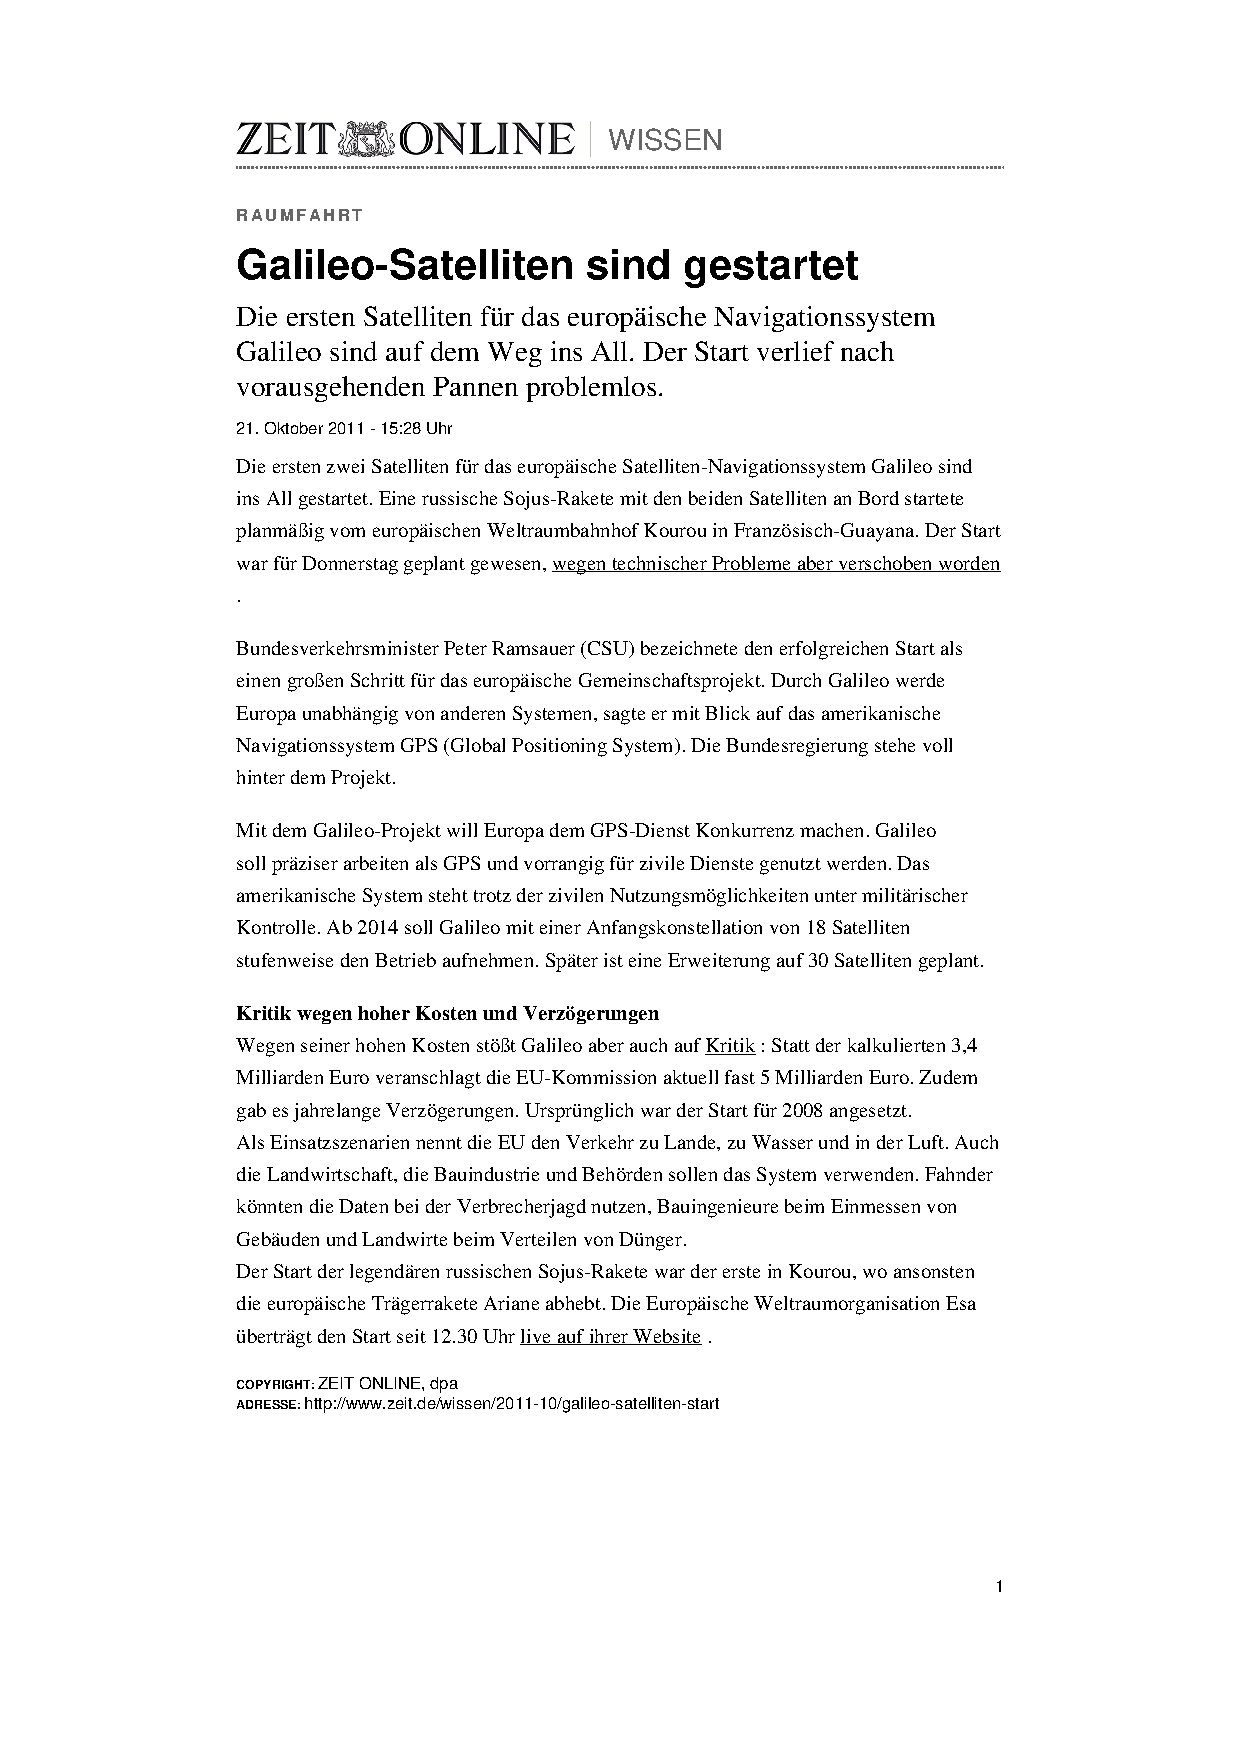
\includepdf[landscape=false, pages=-]{galileo-satelliten-start.pdf}

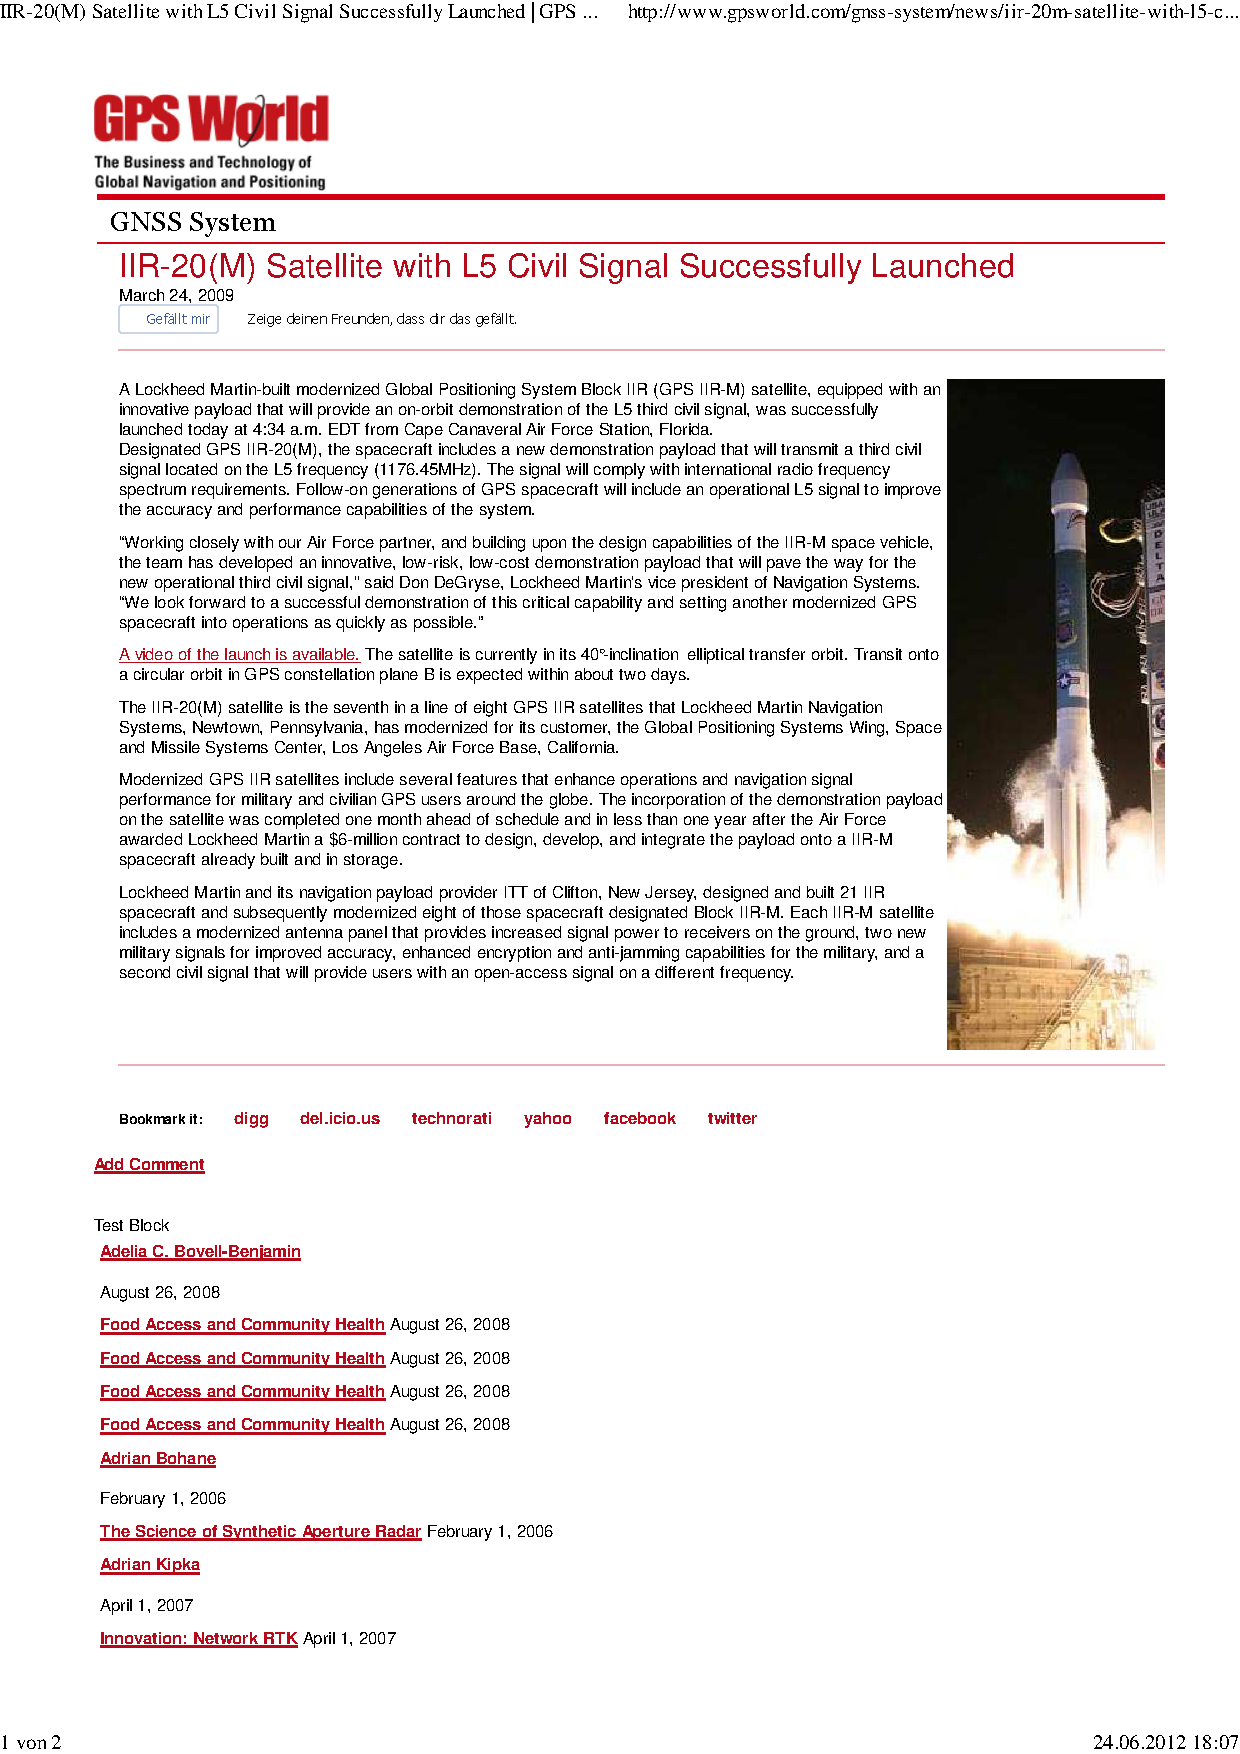
\includepdf[landscape=false, pages=-]{gps_world_article.pdf}


\includepdf[landscape=false, pages=-]{gps_europe.pdf}


\chapter{Vortrag Rechtliches}
\label{index:vortrag-rechtliches}

\section{Präsentation Rechtliches}
\label{included_projects/rechtliches/RECHTLICHES_SPEC/appendix:prasentation-rechtliches}\label{included_projects/rechtliches/RECHTLICHES_SPEC/appendix::doc}
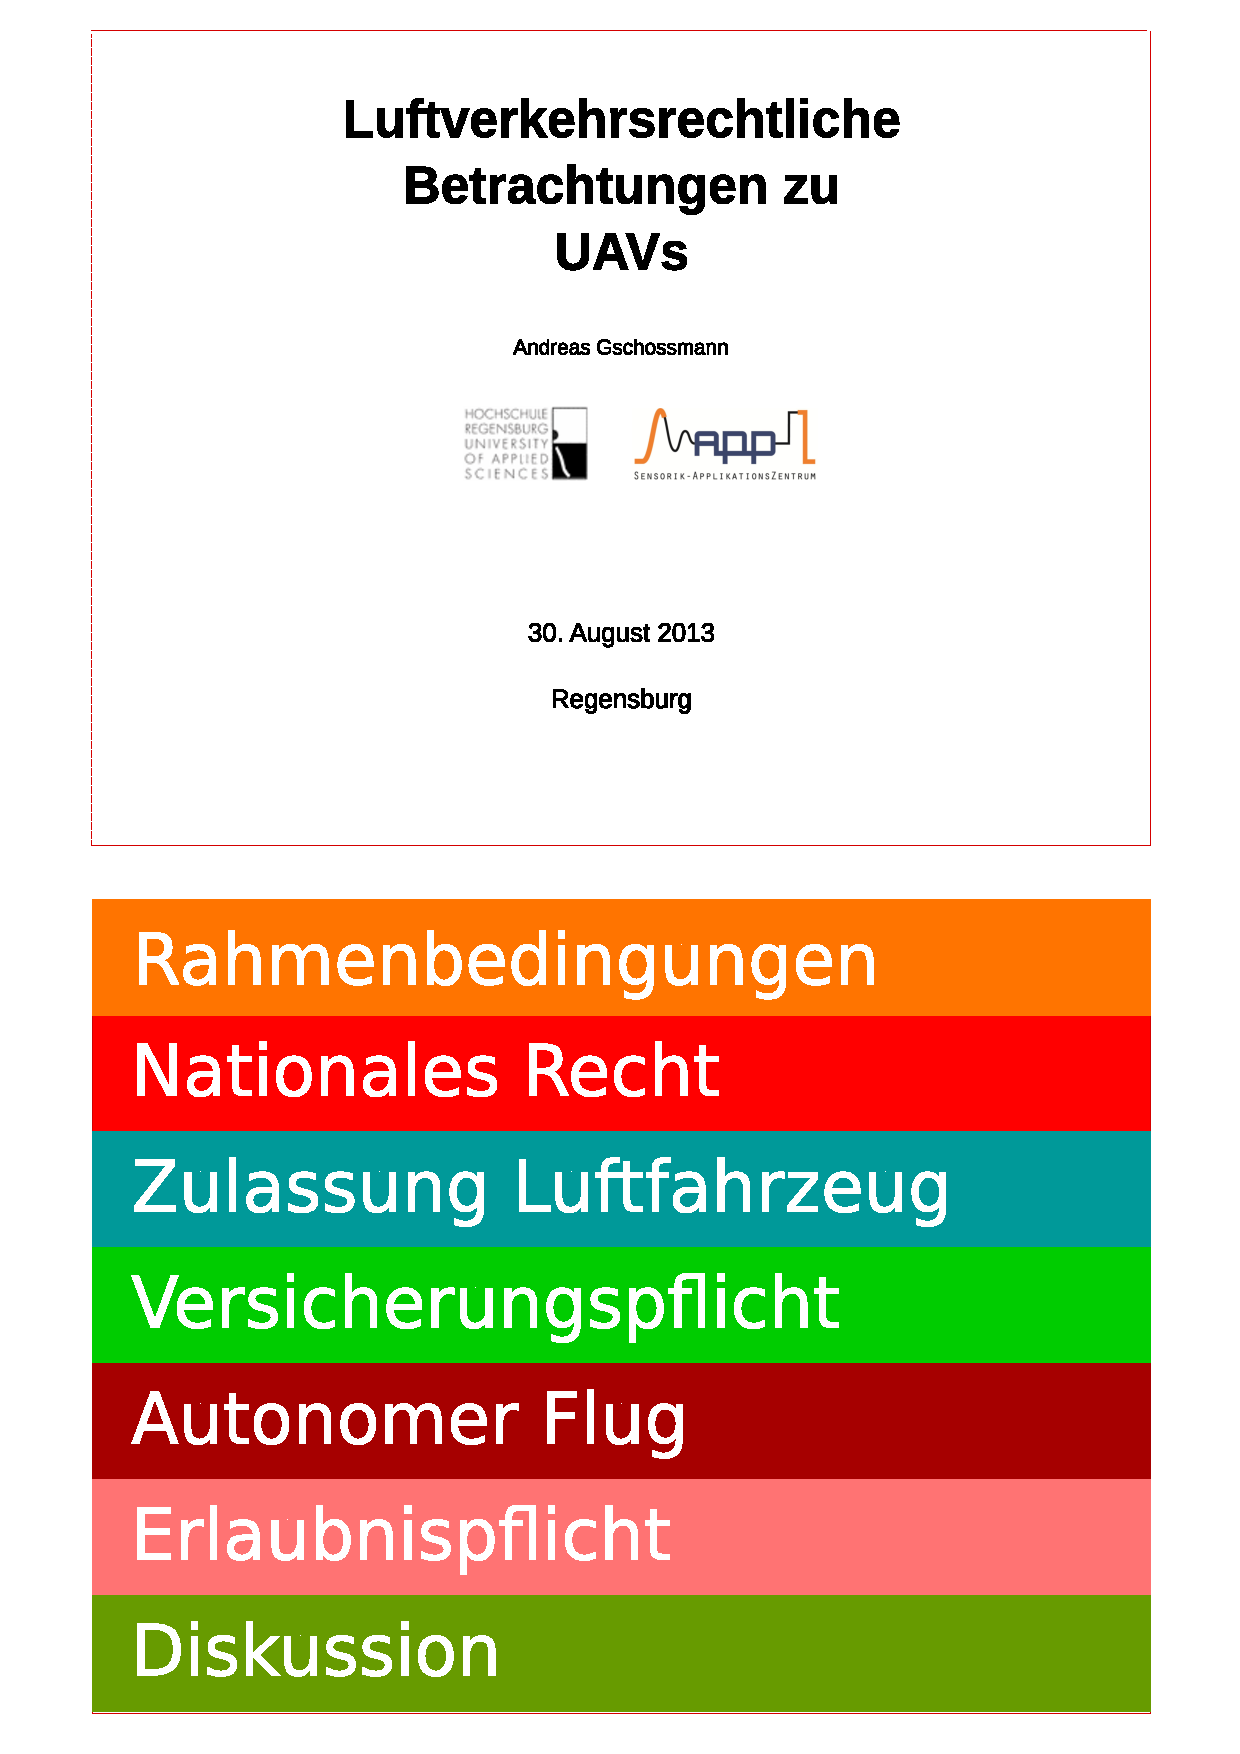
\includepdf[landscape=false, pages=-]{rechtliches.pdf}
\end{appendix}
%\addtocontents{toc}{\protect\setcounter{tocdepth}{2}}

\bibliographystyle{plain}
\bibliography{GPS_SPEC,RECHTLICHES_SPEC}


\renewcommand{\indexname}{Stichwortverzeichnis}
\printindex
\end{document}
